\documentclass[11pt]{article}

\usepackage{graphicx}
\usepackage{amsfonts}
\usepackage{amsmath}
\usepackage{amsthm}
\usepackage{latexsym}
\usepackage{amssymb}
\usepackage{hyperref}


\newtheorem{theorem}{Theorem}[section]
\newtheorem{lemma}[theorem]{Lemma}
\newtheorem{corollary}[theorem]{Corollary}
\newtheorem{assumption}[theorem]{Assumption}
\newtheorem{proposition}[theorem]{Proposition}
\newtheorem{observation}[theorem]{Observation}
\newtheorem{defin}[theorem]{Definition}
\newtheorem{definition}[theorem]{Definition}
\newtheorem{example}[theorem]{Example}
\newtheorem{conjecture}[theorem]{Conjecture}
\newtheorem{claim}{Claim}

\pagestyle{plain}
\bibliographystyle{plain}
\graphicspath{ {C:/Users/sam/Desktop/images/} }
\title{DES Algorithm}
\author{}
\date{}

\begin{document}

\maketitle

 
\section{Introduction}
\subsection{Cryptography}
 Study of techniques to make a message into a specific format and transmitting, which could not be read directly without knowing the way to decode it.
In simple words storing and sending data in a form that only intended can read it.


\subsection{History of Cryptography}
The Cryptography came into existence to secure the transmitting data from one place to another. To go to the history of cryptography its long way back to 1900 B.C\cite{History} when An Egyptian Sculpture was found this was documented as the first cryptography.
It traveled through lot of forms like using the signatures, ATBASH (substituting alphabets), skytale(using a stick with specified length and wrap the message around it to read), Julius Caesar(similar to ATBASH but a bit different it uses shift by 3 for example in place of A, D is used).A.D Abu (using some crypt in a plain text), later nomenclator (using different words for hiding important names etc).  


The encryption came into existence long back, to go to history it’s a long way back in 1900 B.C , it was  mostly used during wars.  Need of Digital Cryptography came into existence with Telegraph which made United States a Communication power.

In 1844 until world war 2 the cryptography is only used for military and government purposes. Post-war many businesses started using this for encrypting their data for making it safe from competitors.

In this days everyone one wants securing data from the third party where this would not be complete without consideration of encryption technology.Encryption means obscuring the meaning of data by converting it into some secrete code such that can only be decoded and understood by people whom it is intended.
In 1973, NIST requested for proposals of national-symmetric key cryptosystem. IBM proposed modified version of LUCIFER for the request, which was accepted as DES.A drafted version of DES was published in the Federal register in march 2015. Later in January 1977 DES was published in Federal Register as FIPS 46.


\section{Background}\label{background_label}
The general terms used in DES are:-
\begin{enumerate} 
	\item Symmetric key
	\item Permutationem
	\item left shift
	\item XOR
\end{enumerate}
\subsection{Symmetric Key}
The key that is used for encrypting and decrypting the message is same which mean it uses only a single-key. 
That differs from asymmetric (or public-key) encryption, which uses one key to encrypt a message and another to decrypt the message which means it uses two keys.

\subsection{Permutation}
Arranging of a collection of things or elements in all possible ways with an order
 
Example: You want to watch three movies Adi ("a"), Baahubali ("b") and Chenna ("c"), but haven't decided in what order. What choices do you have?

Answer: \{a,b,c\} \{a,c,b\} \{b,a,c\} \{b,c,a\} \{c,a,b\} \{c,b,a\}

order is important

\subsection{left shift}
 shifts the bits of expression left by the number of bits specified.\newline
 
 
 For Example:-
 
 
 lets take value 14 (2bit-leftshift)
 
 
covert 14 to binary value


 00001110 

 2-bit leftshift

 00111000
 
\subsection{XOR}
The XOR ( exclusive-OR ) gate acts in the same way as the logical "either/or.Outputs true if  any one input is true 
and outputs "flase" if the both the inputs are "flase".

\begin{figure}[h!]
	\begin{center}
		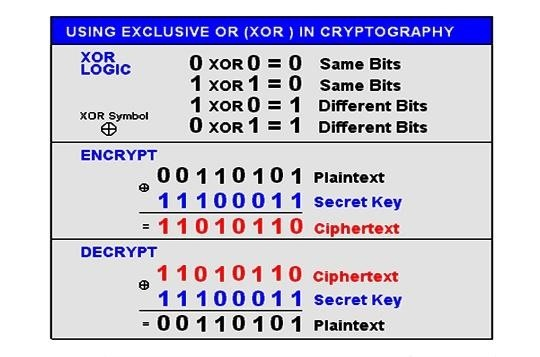
\includegraphics[scale=1.5]{xor}
	\end{center}
	\caption{Truth Table.}\label{nice_figure}
\end{figure}

 \section{Data Encryption Standard (DES) Alogrithm}
 DES\cite{source} is symmettric block cipher,it encrypts 64 bits plain text with 64 bits key and returns output of 64 bits cipher text block .
 The encryption process consists of Three main parts:-\newline
 1.Initial and final permutation\newline
 2.16 Feistel Rounds\newline
 3.Key Generation\newline
  \begin{figure}[h!]
  	\begin{center}
  		\includegraphics[scale=0.9]{Des1}
  	\end{center}
  	\caption{General structure of Des}\label{nice_figure}
  \end{figure}
  
 \subsection{Permutation}
 The given input of 64 bits data M first goes through the initial permutation .This 64 bits data M is rearranged in the  order of following table.
 \begin{figure}[h!]
 	\begin{center}
 		\includegraphics[scale=0.9]{ip}
 	\end{center}
 	\caption{intial permutation}\label{nice_figure}
 \end{figure}

 where 58th bit of M becomes the first bit of Ip and 50th bit becomes the second bit and 7th bit becomes the last bit.
let M be the plain text message M = 1111111111111111, where M is in hexadecimal (base 16) format.
  
  Changing this to binary format\newline
 M=0001000100010001000100010001000100010001000100010001000100010001 
 ip=0000000011111111000000001111111100000000000000000000000000000000\newline
 
 After initial permutation the permuted block ip is divide into two equal parts left half and right half and this under goes 16 feistel rounds.
 \begin{figure}[h!]
 	\begin{center}
 		\includegraphics[scale=0.5]{des2}
 	\end{center}
 	\caption{DES Alogrithm  }\label{nice_figure3}
 \end{figure}
 \newline
 
  Then finally it goes through final permutation which is also know as inverse of initial permutation, where the order is again rearrange in the way as following table
  \begin{figure}[!h]
  	\begin{center}
  		\includegraphics[scale=0.5]{inverse}
  	\end{center}
  	\caption{inverse permutation}\label{nice_figure4}
  \end{figure}
\newline

That is, the output of the algorithm has bit 40 of the preoutput block as its first bit, bit 8 as its second bit, and so on, until bit 25 of the preoutput block is the last bit of the output.
\subsection{Key Genration}
In DES size of the key is 64 bits long but uses 56 bits key to operate on 64 bits data ,where every 8th of the key is not used (bits 8,6,24,32,40,48,56,64).
Let take a hexadecimal key K=1111111111111111.This then converted into binary form
where value of '1'=0001.\newline
k=0001000100010001000100010001000100010001000100010001000100010001\newline 
The Key undergoes different steps  as shown figure
 \begin{figure}[!h]
	\begin{center}
		\includegraphics[scale=0.7]{key}
	\end{center}
	\caption{key genration}\label{nice_figure6}
\end{figure}

where first 64 bits key goes through parity drop and the key is reduced to the 56 bits key where every 8th bit is removes for parity check.\newline
And reaaranged in the order of permuted table.\newpage
\begin{figure}[!h]
	\begin{center}
		\includegraphics[scale=0.5]{pc}
	\end{center}
	\caption{key genration}\label{nice_figure6}
\end{figure}
Now 64 bits is reaaranged to 56 bits permuted key in above order leaving out every 8th bit.
We get,\newline
K=00000000000000000000000011110000000000000000000000001111
 
And now this 56bit key is made into two equal parts 28bit each .and then this left half and right half keys goes through left shift ,where this proccess continued 16 times to create 16 subkeys,each of which is 48-bits long.
\newline
\newline
$C_{0}$=0000000000000000000000001111\newline
$D_{0}$=0000000000000000000000001111
\newline

now we create 16 blocks where every $C_{n}$,$D_{n}$ is obtained from previous pair $C_{n-1}$,$D_{n-1}$ where n=1,2,3......16. now we left shift to obtain the block
where rounds 1,2,9,16 are one bit left shit and the others 3,4,5,6,7,8,10,11,12,13,14,15 are two bit left shift.For example  $C_{1}$,$D_{1}$ are formed from previous $C_{0}$,$D_{0}$ by doing one bit left shift on them.
\newline \newline
$C_{1}$=0000000000000000000000011110
\newline
$D_{1}$=0000000000000000000000011110
Now we get keys $K_{n}$ where n=1,2,...16. Each pair of 56 bits($C_{n}$ $D_{n}$) is reduced to form 48 bits key in compression box,where 56 bits key is rearranged in the order of permuted table.
\newpage
\begin{figure}[!h]
	\begin{center}
		\includegraphics[scale=0.6]{pc2}
	\end{center}
	\caption{Permuted table-2}\label{nice_figure6}
\end{figure}
where each pair of combined $C_{n}$$D_{n}$ is rearanged in the order above \newline
For example: lets take $C_{1}$$D_{1}$\newline
$C_{1}$$D_{1}$=00000000000000000000000111100000000000000000000000011110\newline
Therefore, the first bit of $K_{1}$ is the 14th bit of $C_{1}$$D_{1}$, the second bit the 17th, and so on, ending with the 48th bit of $K_{1}$.In similar way we obtain the rest of the 15keys($k_{2}$ to $K_{16}$) .

\section{Feistel Round}
In DES we have 16 feistel rounds where the rightmost 32 bits data goes through the feistel round as shown in figure4. We are going to know what  happens in the cipher function in detail.
\newline
The following figure shows operation that inside the fiestel round\newline
\begin{figure}[!h]
	\begin{center}
		\includegraphics[scale=0.6]{fei}
	\end{center}
	\caption{Permuted table-2}\label{nice_figure7}
\end{figure}
 
when the one half of 64 bits data that is 32 bits which first goes through expansion p-box where  32 bits data is converted into 48 bits. Where 32 bits data is converted with help of selection table as below.
\begin{figure}[!h]
	\begin{center}
		\includegraphics[scale=0.6]{ebit}
	\end{center}
	\caption{selection table}\label{nice_figure8}
\end{figure}
\newline

The first three bits of the newly generated 48 bits data are  32,1,2 bits of 32 bits and last 2 bits are 31 and 1 of 32 bits.Then we have Xored the result with  48 bits key $K_{n}$ where n=1,2...16.And now we get a output of 48 bits then which goes through S-box (8 s-boxes are used).In s-box we reduce 48 bits to 32 bits this done by dividing 48 bits data into groups of each with 6-bits of data .Each group of six bits will give us an address in a different s-box. Located at that address will be a 4 bit number. This 4 bit value will replace the original 6 bits. Then net result is that the eight groups of 6 bits are transformed into eight groups of 4 bits (the 4-bit outputs from the S boxes) for 32 bits total.
For example lets take 1st group  value be '100110' to understand.
where the value of 1st bit and 6th bit gives value  of the  column of s-box $S_{1}$ that is 2
('10'=2) and the rest 4 bits denotes row value is '0011' is 3. The value in 2nd column and 3rd row of the s-box  $S_{1}$ is 8 this value is converted into 4-bit value that is '1000'. Similarly it is done for rest of the 7 groups of each 6 bits.And reduced to 32 bits by combining the output from all the s-boxes.\newpage
\begin{figure}[!h]
	\begin{center}
		\includegraphics[scale=0.8]{s-boxes}
	\end{center}
	\caption{s-boxes}\label{nice_figure9}
\end{figure}
Now this 32 bits is passed through the straight p-box where order of 32 bits is rearranged as show below to output  32 bits
\begin{figure}[!h]
	\begin{center}
		\includegraphics[scale=0.8]{p}
	\end{center}
	\caption{P-table}\label{nice_figure10}
\end{figure}

Then finally this right 32 bits and left half 32 bits passes through XOR ,the same process repeats 16 times (16 rounds).Where we will have L2 = R1, which is the block we just calculated, and then we must calculate R2 =L1 + f(R1, K2), and so on for 16 rounds. At the end of the sixteenth round we have the blocks L16 and R16. And this L16 and R16 goes through inverse permutation.
\section{Decryption}
This is Exactly reverse functioning of Encryption where inverse permutation will be fist and intial permutation will be final.All the keys that are created while encryption are  stored and used in reverse order .
\begin{figure}[!h]
	\begin{center}
		\includegraphics[scale=0.8]{de}
	\end{center}
	\caption{P-table}\label{nice_figure11}
\end{figure}
\section{Drawbacks}
1.DES fails in front of linear crypt-analysis, because during its design this   attack wasn't invented.Now in the age of parallel computing, breaking DES has become easy   with the help of brute force attack which was impossible during that time.\newline
2.There can be same output from the S-Boxes on different inputs on permutation. These are called Semi weak  keys.\newline
3.The usage of intial and final permutation are not clear.\newline
4.If the message is encrypted with a  particular key, and is taken 1’s compliment of that encryption will be same as that of the encryption of the compliment message and compliment key.
\bibliography{my_sources}
\end{document}

